\documentclass[../main.tex]{subfiles}

\begin{document}

\section{Use Case Description}
\label{section:problem:use_case}
\begin{figure}[h]
    \centering
    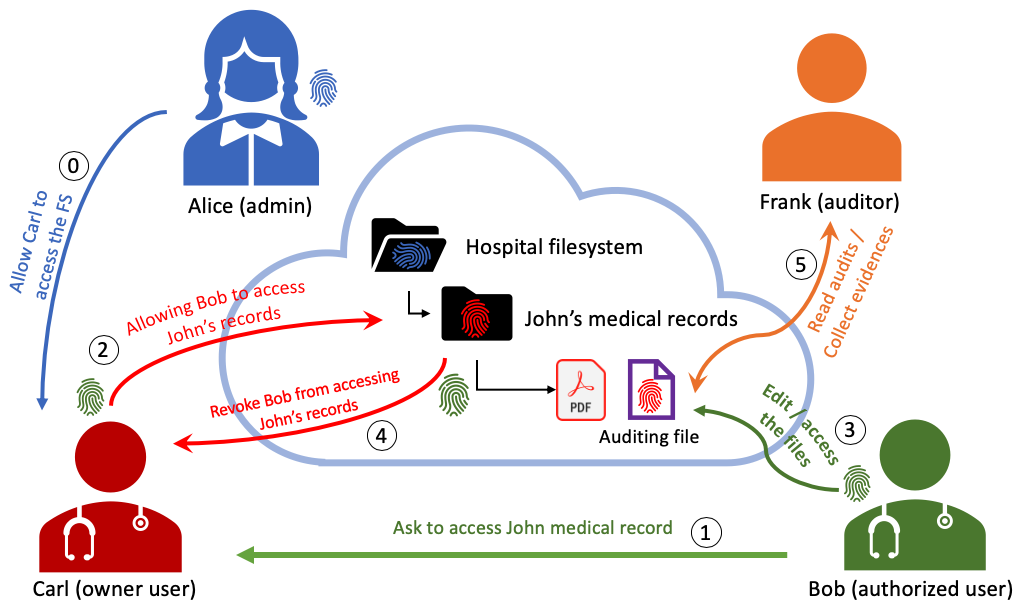
\includegraphics[width=0.75\textwidth]{../../images/problem/use_case}
    
    \label{figure:problem:use_case}
    \caption{Use case representation}
\end{figure}

\par Before going deeper in the protocol description we will first take a look of at higher level use case presented in the Figure \ref{figure:problem:use_case}. First of all, as explained in Section \ref{section:problem:overview}, we see that the resource shared between parties is what we call a filesystem. Furthermore, we see that there are three parties intervening, each of them having a specific role. In order to explain each role, we are going to look at the scenario and explain one step at a time what is its purpose and who are the actors.

\par At first, we have Bob, the authorised user who needs to access a specific file or folder of the filesystem, John's medical record in this case. In order to do so, Bob must first be authorised by the owner user, Carl. Carl will allow Bob to access this directory by linking Bob's fingerprint (the green fingerprint in Figure \ref{figure:problem:use_case}) to the target. In this way, Bob can now access the target when representing its own fingerprint.
\par Once allowed, Bob can do whatever required actions (in the range set by Carl) at the condition that he specifies the purposes of each of them. Those intent are stored in an auditing file linked every accessed file within the target directory. When Bob no longer needs to access John's records, Carl can simply remove its fingerprint from the target folder thereby preventing Bob to access newer versions of this directory.
\par Lastly, in a case of a GDPR inspection, an auditor, Frank, can retrieve and analyse the auditing files linked to John's records. Theses auditing files list all the operations made by users to a file, along with contextual information like the justification, the date/time and so on.

\end{document} 